\section{Auditing and Recovering Rebuilt Workloads}
\label{sec:recovery-results}

\subsection{RQ3: What Does the Audit Actually Authorize?}
Auditing unshifted source reuse rejects every candidate and routes all 20 target decisions to the endpoint in the original replay. The audit therefore prevents cheap but unqualified reuse, yet recovers no search saving by itself. Target-selection recalibration changes the candidate before certification. The original procedure accepts 19 of 20 recalibrated candidates; Arxiv seed 1229 has candidate UCB 0.05056 and falls back despite being close to the threshold.

The joint-error sensitivity is more selective (Figure~\ref{fig:decisions}). With $\alpha_c=\alpha_e=0.025$, it accepts all ten SIFT candidates and six Arxiv candidates. All twenty endpoints pass their allocated checks, so four Arxiv decisions fall back and none abstains. The final decision satisfies the per-target construction in Proposition~\ref{prop:simultaneous}, subject to its query-sampling conditions. Certification rejection is not a finding of true unsafety: it changes the supported action given the available 500-query certificate.

\begin{figure*}[t]
\centering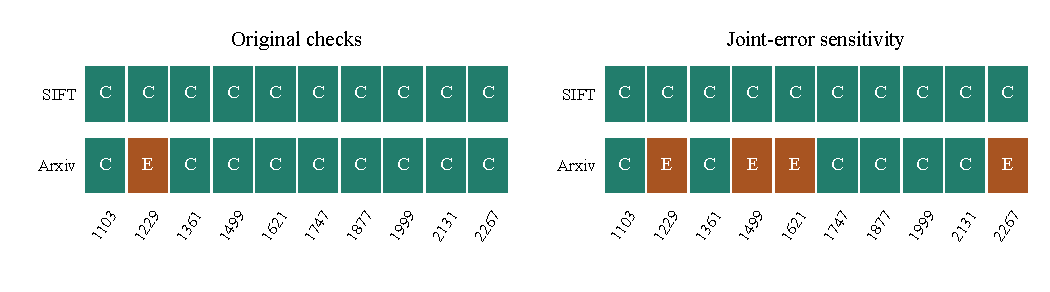
\includegraphics[width=\textwidth]{figures/decisions.pdf}
\caption{One cell per target decision, ordered by registered seed rather than a time axis. C: candidate accepted; E: endpoint fallback. Left: original two individual 95\% checks. Right: post-hoc 0.025+0.025 joint-error allocation. The same selected shifts and certification queries are used in both. Candidate acceptance falls from 19/20 to 16/20, while every completed decision remains qualified by its corresponding endpoint or candidate check.}
\label{fig:decisions}
\Description{SIFT accepts ten candidates under both rules. Arxiv accepts nine under the original rule and six under the joint-error rule; other cells use the endpoint.}
\end{figure*}

\subsection{RQ4: How Much Search Efficiency Is Recovered?}
Recalibration restores substantial search efficiency within the recurring-profile workload (Table~\ref{tab:recovery}). The original decisions reduce risk to 1.79\% and 2.04\%, with relative mean-NDC reductions of 44.39\% and 44.79\%. Crossed resampling widens SIFT's interval compared with the old independently-within-build procedure: it is now [42.76, 46.01]\%, rather than [43.88, 44.91]\%. Preserving shared query dependence changes uncertainty even when the point estimate is unchanged.

\begin{table*}[t]
\caption{Completed refresh decisions on ten targets and 1,000 evaluation queries per target. Query risk and relative mean-NDC reduction are percentages [crossed 95\% interval]; intervals are conditional on fixed source histories and selected shifts. Original and joint-error rows differ only in certification composition. All fallback executions are included. Mean and p95/p99 are distance calculations, not latency.}
\label{tab:recovery}
\small\begin{tabular*}{\textwidth}{@{\extracolsep{\fill}}llrrrrr@{}}\toprule
Dataset & Decision & Risk [95\% interval] & Reduction [95\% interval] & Mean NDC & p95 & p99\\\midrule
\RecoveryRows
\bottomrule\end{tabular*}
\end{table*}

Under the joint-error allocation, SIFT is unchanged, while Arxiv risk becomes 1.68\% and relative mean-NDC reduction becomes 29.86 [14.75, 45.00]\%. Figure~\ref{fig:tradeoff} shows that stricter qualification moves the decision toward the endpoint: it reduces risk and sacrifices some efficiency. The positive intervals support recovery of useful search work on both datasets, not a claim of optimality over adaptive-search methods with different information budgets. In particular, the comparator here is the same graph's fixed endpoint, not the best target-trained method.

\begin{figure}[t]
\centering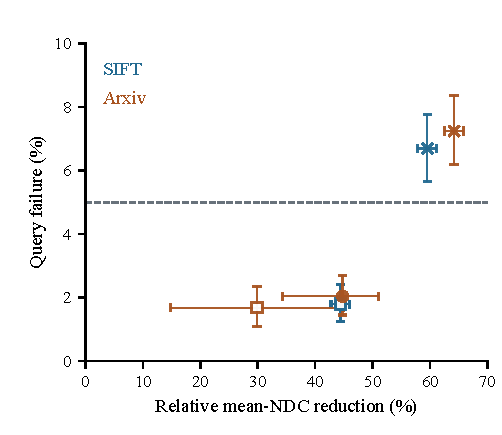
\includegraphics[width=\linewidth]{figures/tradeoff.pdf}
\caption{Refresh risk--work tradeoff with crossed 95\% intervals. The 5\% line is the query-risk target, not a confidence bound. Filled symbols: original recalibration; open symbols: joint-error replay; crosses: direct reuse. SIFT's original and joint points coincide.}
\label{fig:tradeoff}
\Description{Direct reuse has larger search savings but more than 5 percent failure. Both recalibration rules have lower risk; the joint Arxiv point gives up some work saving.}
\end{figure}

\subsection{RQ4 Boundary and Replication: Can Fixed Slack Transfer?}
\label{sec:fresh-bridge}
The first fresh-query stage tests the source-derived policy of Section~\ref{sec:slack-method}, not TCP. Source certification and 500 held-out target queries are different objects: the former determines the executable candidate, while the latter initially supplies a portability audit rather than a target deployment certificate. The complete three-lane table remains in the supplement. Its main boundary is simple. On hnswlib, the $+1$ lane clips to the endpoint for all registered sources and therefore saves no work on either dataset. On Faiss, the same lane retains 8.27\% and 29.09\% mean-NDC savings, with held-out empirical risks of 0.18\% and 0.67\%; no held-out direction exceeds 5\% empirical risk. This stage fixes a viable candidate family but does not authorize target deployment.

The post-seal replication closes that gap with new, mutually exclusive target certification and evaluation roles (Table~\ref{tab:target-certified}). Every candidate and endpoint has a target CP UCB below 5\%; all 552 directions per dataset deploy the frozen candidate, with no fallback or abstention. The largest candidate certificate counts are 5/500 on SIFT and 6/500 on Arxiv-Nomic (UCBs 2.32\% and 2.59\%). Evaluation risk is 0.126 [0.040, 0.250]\% on SIFT and 0.530 [0.233, 0.915]\% on Arxiv-Nomic. Mean-NDC savings remain 8.283 [7.921, 8.557]\% and 29.083 [28.653, 29.518]\%. These crossed target--query intervals are wider than the target-only intervals but leave the conclusions unchanged. Pooled and worst-target p95 ratios remain below one, and leaving out any target preserves positive mean savings.

\begin{table*}[t]
\caption{Post-seal Faiss target-certified replication. Each dataset has 24 targets, 552 directed decisions, 500 target-certification queries, and 500 disjoint evaluation queries. C/F/A counts candidate, fallback, and abstention decisions. Risk and mean-NDC saving are percentages [95\% crossed target-build/query-ID bootstrap interval]. P95 reports pooled/worst-target ratios to the endpoint; LOTO is the minimum mean saving after deleting one target.}
\label{tab:target-certified}
\small\begin{tabular*}{\textwidth}{@{\extracolsep{\fill}}lrrrrr@{}}\toprule
Dataset & C/F/A & Eval. risk [95\% CI] & NDC saving [95\% CI] & P95 ratio & LOTO saving\\\midrule
\TargetCertifiedRows
\bottomrule\end{tabular*}
\end{table*}

The candidate is below the endpoint in 92/552 SIFT directions and 322/552 Arxiv directions; in the others the upward rung clips to the endpoint. This explains why every decision can deploy the candidate while many isolated directions have zero saving. It also preserves the implementation boundary: no target-certified hnswlib claim is made because the registered hnswlib candidate already equals the endpoint. Fixed-machine interleaved timing points in the same direction (9.27\% and 26.57\% mean reductions), but remains exploratory; NDC is the primary efficiency endpoint.

\subsection{RQ5: Does Recovery Worsen the Search-Work Tail?}
Neither recalibration rule increases query-pooled p95 or p99 relative to the endpoint. For joint-error replay, p95 is 2,349 versus 2,615 NDC on SIFT, and 3,117 versus 3,252 on Arxiv; p99 is 2,774 versus 2,855 and 3,460 versus 3,504. Every individual target also has non-increasing p95 and p99. Figure~\ref{fig:tails} displays the per-target ratios without connecting unrelated seeds.

\begin{figure}[t]
\centering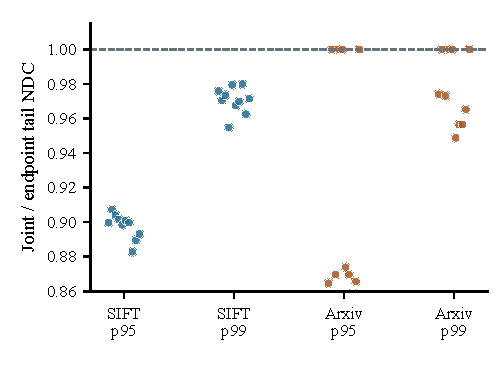
\includegraphics[width=\linewidth]{figures/tails.pdf}
\caption{Per-target tail ratios for joint-error replay, relative to that target's endpoint; ten dots per dataset/quantile. Equality reflects an endpoint fallback. All ratios are at most one. These descriptive tail comparisons are not formal noninferiority certificates or wall-clock results.}
\label{fig:tails}
\Description{Paired target p95 and p99 ratios fall at or below the equality line; endpoint fallback targets have ratio one.}
\end{figure}

The fallback is a build-level choice, so its serving distribution is exactly the fixed endpoint's distribution for that build. Combining it with candidate-serving builds can change pooled quantiles even without changing a candidate's query path. Reporting both pooled and per-target tails avoids hiding this composition effect. It also avoids inferring tail behavior from the much larger mean gain alone.

\subsection{RQ6: Is the Benefit Driven by One Target?}
The minimum LOTO mean-NDC reduction is 44.37\%/44.23\% for original SIFT/Arxiv decisions, and 44.37\%/27.64\% for joint-error decisions. Deleting the largest relative-gain build produces those same minima in these records. These are overlapping checks, not independent confirmations. Target-only and shared-query-only interval sensitivities in the supplement show different uncertainty sources: SIFT's variation is dominated by queries, whereas Arxiv's stricter-rule result also varies strongly with the candidate/fallback choice across targets. The retained positive direction supports a fixed-target-set recovery finding; it does not certify an unseen rebuild distribution.
